\chapter{Valores experimentales} \label{implementacion}
En este capítulo se expondrán los resultados de los experimentos realizados, creando una apartado por algoritmo. Se estudiará: como afectan la cantidad de bits al proceso de cuantificación, si hay diferencia de rendimiento final al aplicar distintas funciones de cuantificación (ASYMM \ref{asymm} y SYMM\ref{symm}), si aplicar la cuantificación a nivel local mejora el nivel global, y como afecta la anchura y la profundidad al rendimiento de las redes cuantificadas.

\newpage

\section{Backpropagation}
El Backpropagation es nuestro algoritmo base de comparación. En este apartado veremos como afecta la cuantificación a este algoritmo.

\subsection{Arquitectura Base}

La comparación entre las funciones de cuantificación se ha realizado sobre el modelo base de 1 capa y 4 neuronas por capa.

\begin{figure}[H]
    \centering
    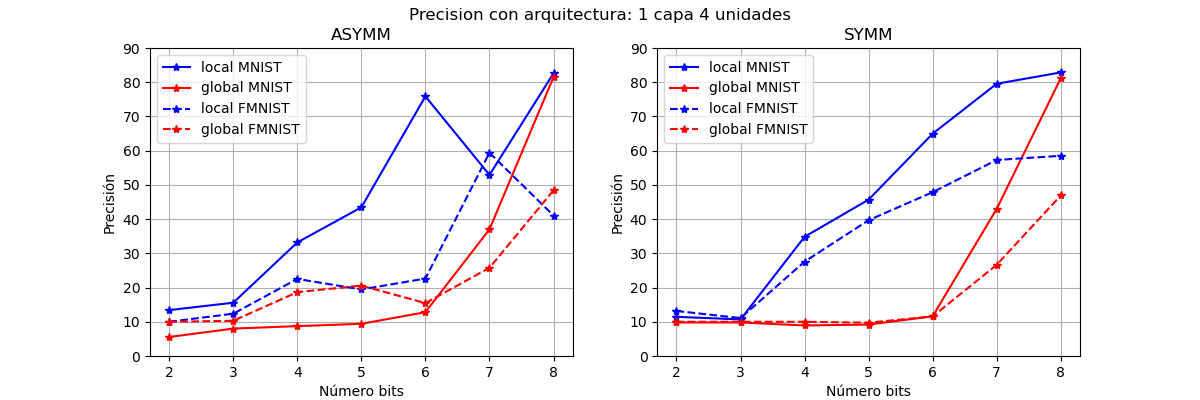
\includegraphics[width=\textwidth]{imagenes/backprop/Precision con arquitectura: 1 capa 4 unidades.png}
    \caption{ASYMM vs SYMM}
    \label{fig:asymmvssymm}
\end{figure}

En esta dos gráficas se representan el rendimiento del modelo base usando la función de cuantificación ASYMM (gráfica de la izquierda) y SYMM (gráfica de la derecha). Cada una de las funciones se ha probado variando la cantidad de bits a usar y el nivel al que se aplica la cuantificación.  

\subsubsection{ASYMM}

Observando los resultados de los modelos entrenados con ASYMM, podemos apreciar como hay una tendencia a mejorar la precisión conforme aumenta el número de bits usados. Si nos fijamos en las precisiones que alcanzan los modelos sobre los conjuntos de datos, se consiguen mejores resultados sobre MNIST que sobre FMNIST. Esto se debe a que (como habíamos definido en \ref{conjuntos de datos}) el problema FMNIST es más complejo y por lo tanto, más difícil de aprender. Centrándonos en el problema MNIST, vemos que la cuantificación local es superior a la global, por lo tanto, la restricción de valores afecta negativamente al rendimiento de los modelos cuantificados. A partir de los 6 bits, los modelos locales empiezan a conseguir precisiones razonables, sin embargo, el modelo de 7 bits tiene peor desempeño que el modelo de 6 bits. ¿Qué ha podido ocurrir? Fijémonos en los entrenamientos de los modelos de 6, 7 y 8 bits.

\begin{figure}[H]
    \centering
    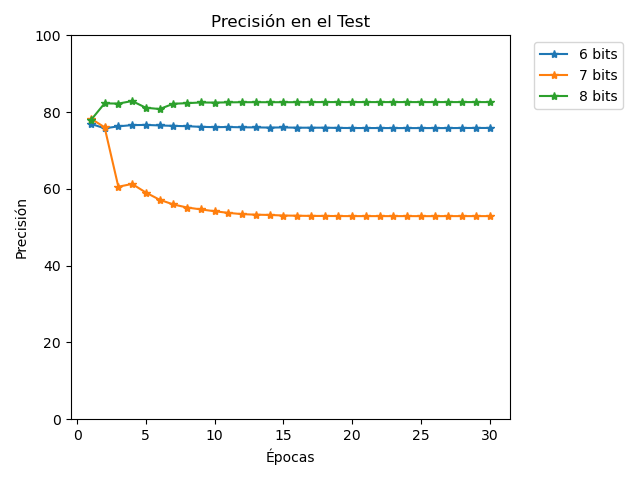
\includegraphics[width=0.75\textwidth]{imagenes/backprop/678bits.png}
    \caption{Entrenamiento de los modelos de 6, 7 y 8 bits}
    \label{fig:my_label}
\end{figure}

Todos los modelos en su primera época consiguen alcanzar un precisión ligeramente alta, en torno al 80\%. Conforme pasan las épocas, los modelos de 6 y 8 bits se quedan en este óptimo, pero el modelo de 7 bits diverge y se estanca en un óptimo peor del que no puede salir. Este fenómeno se puede dar debido al ruido que introduce el proceso de cuantificación. Cuanto más se reduce la precisión numérica, mayor es este ruido. Sin embargo, el modelo de 6 bits no llega a divergir. Este fenómeno se puede dar debido a que al tener menor precisión, el ruido introducido es de menor tamaño que la resolución mínima numérica. Por lo tanto, no perturba el resultado final, actuando como un regulador. 

Volviendo a la gráfica \ref{fig:asymmvssymm} vemos que sobre el conjunto FMNIST se producen las mismas tendencias que en MNIST. Los modelos con cuantificación local consiguen mejores resultados que los que usan la cuantificación global. Sin embargo, con esta arquitectura, los modelos cuantificados no son capaces de conseguir resultados razonables, necesitando la máxima precisión numérica (8 bits) para llegar a rozar el 50\% de precisión. Por lo tanto, se necesita una arquitectura de mayor tamaño que ofrezca una solución mas compleja.

\subsubsection{SYMM}

Al igual que ocurre en los modelos entrenados con la función ASYMM, conforme se aumenta número de bits también aumenta la precisión de los modelos. Con respecto a los conjuntos de datos y niveles de cuantificación, también sucede lo mismo. Se consiguen mejores resultados en MNIST debido a su mayor sencillez. La cuantificación a nivel local es superior a la global debido a que no se reduce el espacio de búsqueda de soluciones. Sin embargo, existe una ligera diferencia entre ambas funciones. Y es que la mejora conforme se aumenta la precisión numérica es más estable que en los modelos que emplean ASYMM. De aquí podemos intuir que los procesos de entrenamiento con cuantificación simétrica tienden a ser menos ruidosos.

\subsection{Arquitecturas grandes}
A continuación, se van a mostrar las precisiones alcanzadas por los modelos con mayor profundidad y anchura.

\begin{figure}[H]
    \centering
    \begin{subfigure}[H]{0.475\textwidth}
    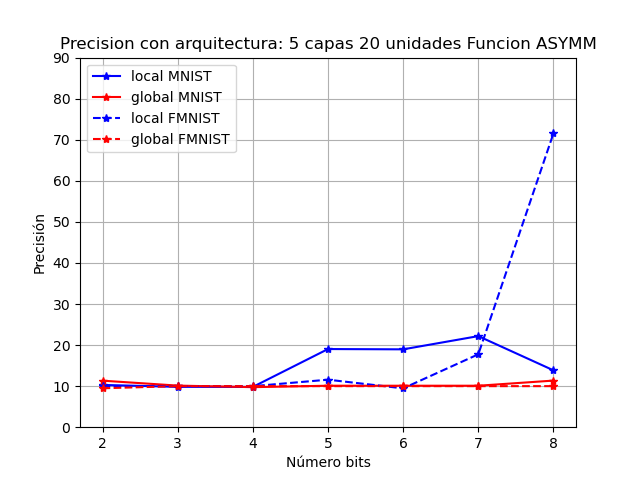
\includegraphics[width=\textwidth]{imagenes/backprop/Precision con arquitectura: 5 capas 20 unidades Funcion ASYMM.png}
    \end{subfigure}
    \begin{subfigure}[H]{0.475\textwidth}
    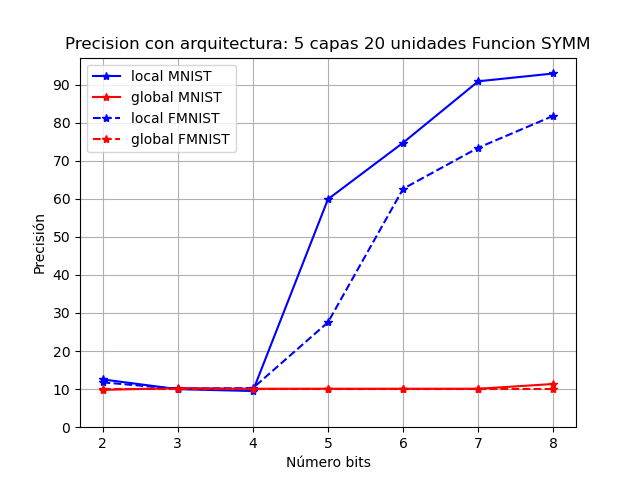
\includegraphics[width=\textwidth]{imagenes/backprop/Precision con arquitectura: 5 capas 20 unidades Funcion SYMM.png}
    \end{subfigure}
    \caption{Arquitectura 5 capas 20 unidades}
    %\label{fig:my_label}
\end{figure}

En esta arquitectura se han aumentado profundidad para ver como

Con esta arquitectura podemos ver como afecta un aumento de la profundidad a las redes cuantificadas. Para ambas funciones, la cuantificación global es inviable. Sin embargo, la cuantificación local si que difiere de una una función a otra. Para la función ASYMM podemos ver que en ambas funciones se consiguen resultados pésimos. A excepción de cuando se usan 8 bits en la función FMNIST, que se alcanza un óptimo del 70\%. Este valor se ha podido dar simplemente porque en la búsqueda a dado con un buen óptimo y se ha quedado ahí estancado.  

Por su parte, los modelos cuantificados con SYMM a nivel local, consiguen resultados decentes en ambos problemas a partir de los 6 bits.

Visto como afecta un aumento significativo de la profundidad a los modelos cuantificados, vamos a explorar como afecta el aumento de la anchura. Para ello haremos uso de modelos con 2 y 3 capas de profundidad a las que aumentaremos en anchura para ver si se mejoran o no los resultados.

Empezaremos por los modelos con 2 capas ocultas.

\begin{figure}[H]
    \centering
    \begin{subfigure}[H]{0.475\textwidth}
    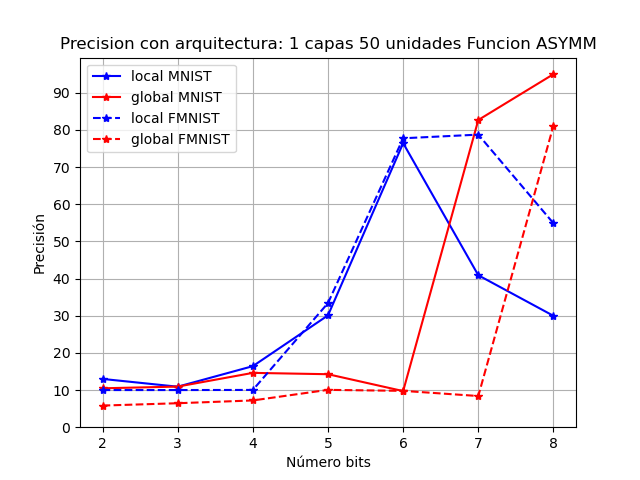
\includegraphics[width=\textwidth]{imagenes/backprop/Precision con arquitectura: 1 capas 50 unidades Funcion ASYMM.png}
    \end{subfigure}
    \begin{subfigure}[H]{0.475\textwidth}
    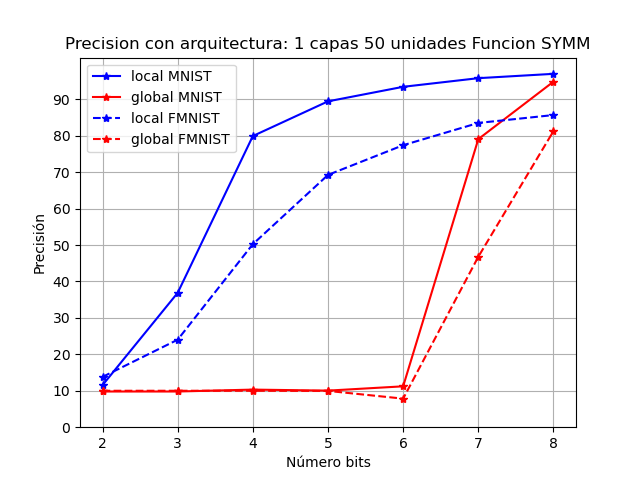
\includegraphics[width=\textwidth]{imagenes/backprop/Precision con arquitectura: 1 capas 50 unidades Funcion SYMM.png}
    \end{subfigure}
    \begin{subfigure}[H]{0.475\textwidth}
    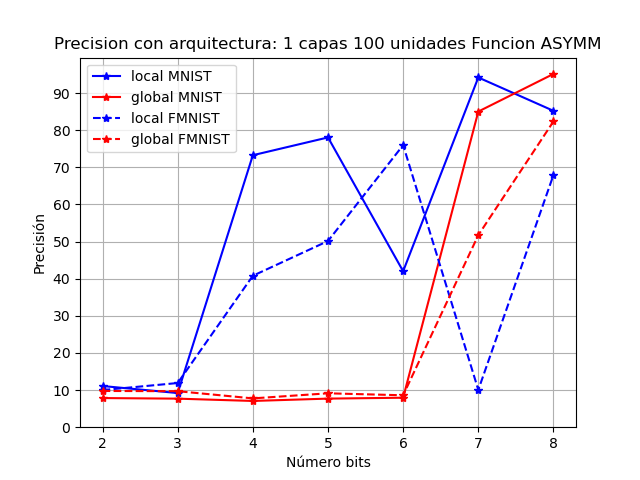
\includegraphics[width=\textwidth]{imagenes/backprop/Precision con arquitectura: 1 capas 100 unidades Funcion ASYMM.png}
    \end{subfigure}
    \begin{subfigure}[H]{0.475\textwidth}
    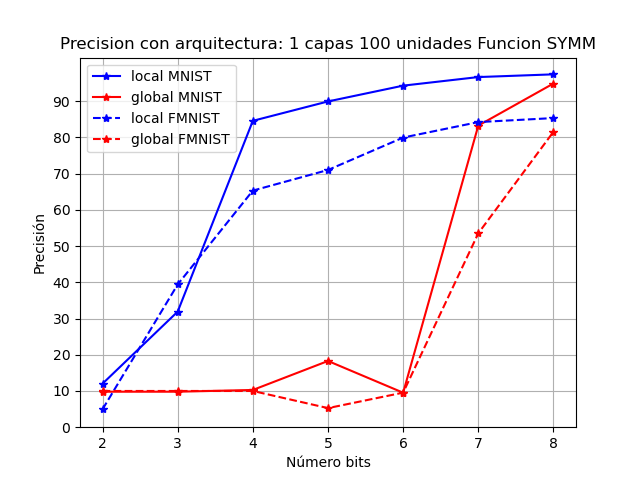
\includegraphics[width=\textwidth]{imagenes/backprop/Precision con arquitectura: 1 capas 100 unidades Funcion SYMM.png}
    \end{subfigure}
    \caption{Arquitectura: 2 capas ocultas}
    %\label{fig:my_label}
\end{figure}

Con este aumento de anchura se pueden ver claras diferencias entre ambas funciones de cuantificación. Los modelos que usan la función ASYMM tienen una clara inestabilidad en la búsqueda de óptimos. Aumentar el número de bits aumenta la capacidad de los modelos para encontrar mejores óptimos, pero no asegura encontrarlos. Esto se puede apreciar en los picos de bajada de las gráficas de la izquierda. Por su parte los modelos que usan las funciones de cuantificación SYMM, son mucho más estables y a mayor número de bits, mayor precisión tienen los modelos. Se sigue cumpliendo que la cuantificación local es superior a la global. Con cuantificación local a partir de los 4 bits se consiguen modelos decentes, mientras que para la cuantificación global se necesitan 8 bits para tener resultados decentes. Con respecto a la diferencia de profundidades vemos que hay una ligera superioridad a los modelos con anchura de 100 unidades. Siendo los modelos con 4 bits donde más se nota esta diferencia.

Ahora vamos a ver lo que ocurre si añadimos una capa oculta más a los modelos.

\begin{figure}[H]
    \centering
    \begin{subfigure}[H]{0.475\textwidth}
    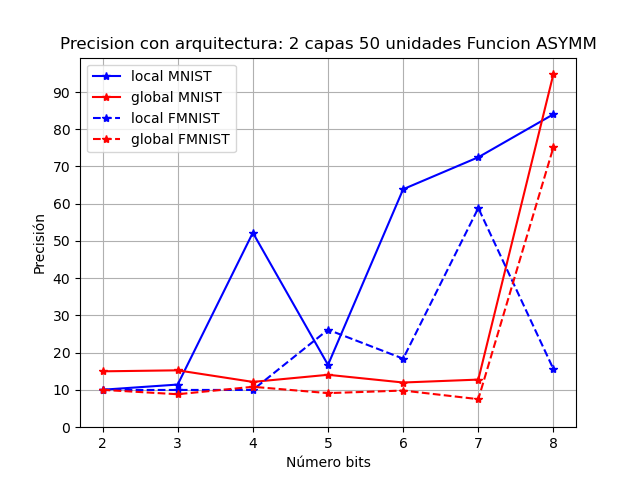
\includegraphics[width=\textwidth]{imagenes/backprop/Precision con arquitectura: 2 capas 50 unidades Funcion ASYMM.png}
    \end{subfigure}
    \begin{subfigure}[H]{0.475\textwidth}
    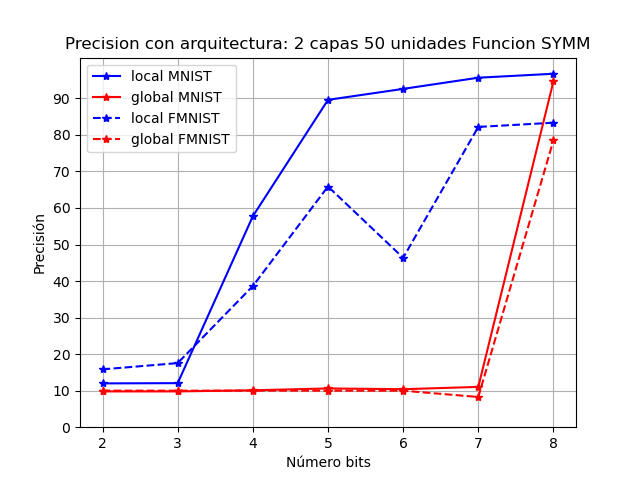
\includegraphics[width=\textwidth]{imagenes/backprop/Precision con arquitectura: 2 capas 50 unidades Funcion SYMM.png}
    \end{subfigure}
    \begin{subfigure}[H]{0.475\textwidth}
    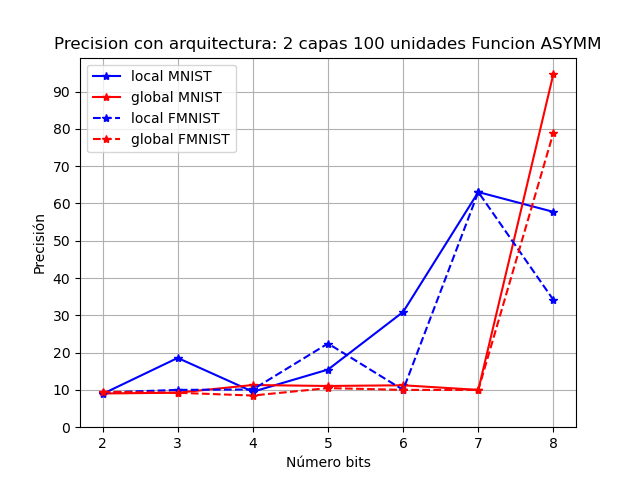
\includegraphics[width=\textwidth]{imagenes/backprop/Precision con arquitectura: 2 capas 100 unidades Funcion ASYMM.png}
    \end{subfigure}
    \begin{subfigure}[H]{0.475\textwidth}
    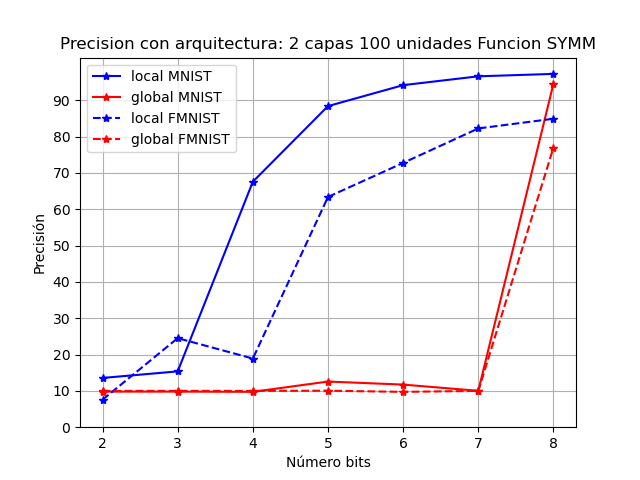
\includegraphics[width=\textwidth]{imagenes/backprop/Precision con arquitectura: 2 capas 100 unidades Funcion SYMM.png}
    \end{subfigure}
    \caption{Arquitectura: 3 capas ocultas}
    %\label{fig:my_label}
\end{figure}

En los modelos cuantificados con la función ASYMM, sigue ocurriendo lo mismo que en los modelos con dos capas. Se mejora la precisión al aumentar el número de bits, pero no siempre ocurre. Debido al ruido, los modelos divergen y no son capaces de encontrar óptimos. Por su parte, los modelos cuantificados mediante SYMM localmente siguen teniendo mejores resultados. A mayor número de bits, mayor precisión. El modelo con anchura de 100 unidades sigue siendo superior al de 50 unidades, obteniendo precisiones más elevadas cuando se disminuye el número de bits. Por su parte, los modelos con cuantificación global necesitan 8 bits para poder tener resultados decentes.

\newpage
\section{HSIC}
En este apartado vamos a analizar el comportamiento del algoritmo HSIC.

\subsection{Arquitectura base}

\begin{figure}[H]
    \centering
    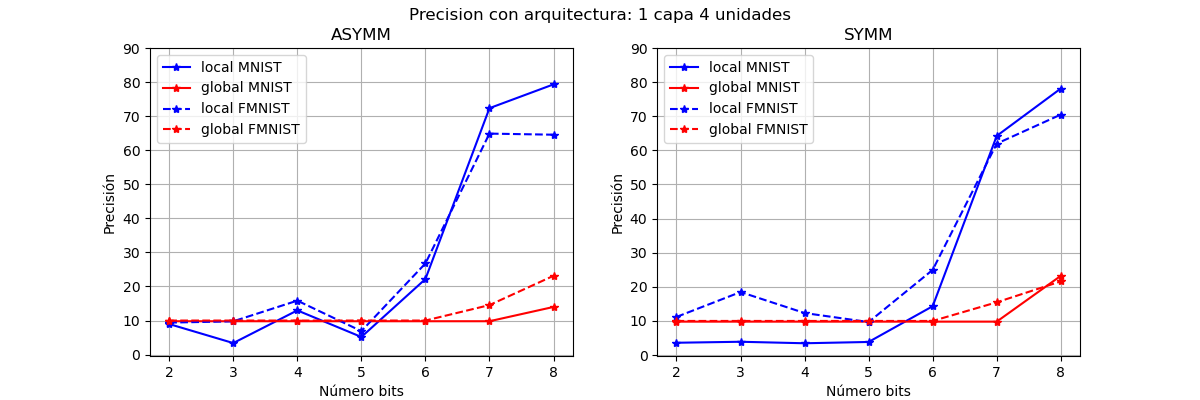
\includegraphics[width=\textwidth]{imagenes/HSIC/Precision con arquitectura: 1 capa 4 unidades.png}
    \caption{ASYMM vs SYMM}
    \label{fig:asymmvssymmHSIC}
\end{figure}

A diferencia de lo que ocurría con el algoritmo de Backpropagation, las gráficas de ambas funciones son prácticamente idénticas. En ambas se ve que con el aumento de la precisión numérica consigue mejorar la precisión de los modelos. Debido a la poca diferencia que hay entre las funciones, voy a realizar el análisis del comportamiento del modelo base sin diferenciar la función de cuantificación a usar.

Con respecto a los problemas tratados, se vuelve a cumplir que los mejores resultados se obtienen en MNIST, debido a su sencillez. Donde si que hay una mayor diferencia es en el nivel al que se aplica la cuantificación. En este algoritmo la cuantificación global hace imposible el aprendizaje. Además, la cuantificación local necesita de una precisión de 7 bits (mayor a la necesitada por el Backpropagation) para tener resultados un poco más decentes. Para intentar comprender por qué este algoritmo se ve tan afectado por la cuantificación global vamos a consultar los máximos y mínimos alcanzados por los pesos de los modelos.

\begin{filecontents*}{pesos_cuantificados_HSIC.csv}
nbits,vmin,vmax,pmin,pmax
6,0.10612637216194444,0.7505927270285349,-1.0,1.0
7,0.07156704797930728,0.8307970218884418,-1.0,1.0
8,0.08083975237842872,0.8025783755120399,-1.0,1.0
\end{filecontents*}
\begin{table}[H]
    \centering
    \begin{tabular}{p{0.15\textwidth}|p{0.15\textwidth}|p{0.15\textwidth}|p{0.15\textwidth}|p{0.15\textwidth}}%
        \bfseries Número bits & \bfseries Varianza mínimo & \bfseries Varianza máximo & \bfseries Peso mínimo & \bfseries Peso máximo% specify table head
        \csvreader[head to column names]{pesos_cuantificados_HSIC.csv}{}% use head of csv as column names
        {\\\hline\nbits & \num{\vmin} & \num{\vmax} & \pmin & \pmax}% specify your coloumns here
    \end{tabular}
    \caption{Información de los pesos cuantificados}
\end{table}

\begin{filecontents*}{pesos_sin_cuantificar_HSIC.csv}
nbits,vmin,vmax,pmin,pmax
6,7786.208395191232,11660.132846061279,-1250.587646484375,1340.1875
7,4331.579097164523,9098.986329433144,-1002.5652465820312,1239.85498046875
8,5846.484648326627,8003.492526127619,-984.1151733398438,1209.60302734375
\end{filecontents*}
\begin{table}[H]
    \centering
    \begin{tabular}{p{0.15\textwidth}|p{0.15\textwidth}|p{0.15\textwidth}|p{0.15\textwidth}|p{0.15\textwidth}}%
        \bfseries Número bits & \bfseries Varianza mínimo & \bfseries Varianza máximo & \bfseries Peso mínimo & \bfseries Peso máximo% specify table head
        \csvreader[head to column names]{pesos_sin_cuantificar_HSIC.csv}{}% use head of csv as column names
        {\\\hline\nbits & \num{\vmin} & \num{\vmax} & \num{\pmin} & \num{\pmax}}% specify your coloumns here
    \end{tabular}
    \caption{Información de los pesos sin cuantificar}
\end{table}

Como podemos apreciar, en este algoritmo, los pesos tienden a tener valores bastantes grandes, por lo tanto, si fijamos el rango de valores entre -1 y 1, el algoritmo no será capaz de alcanzar óptimos. 

\subsubsection{Arquitecturas grandes}

Al igual que en el Backpropagation, primero vamos a analizar como afecta el aumento de la profundidad al modelo.
\begin{figure}[H]
    \centering
    \begin{subfigure}[H]{0.475\textwidth}
    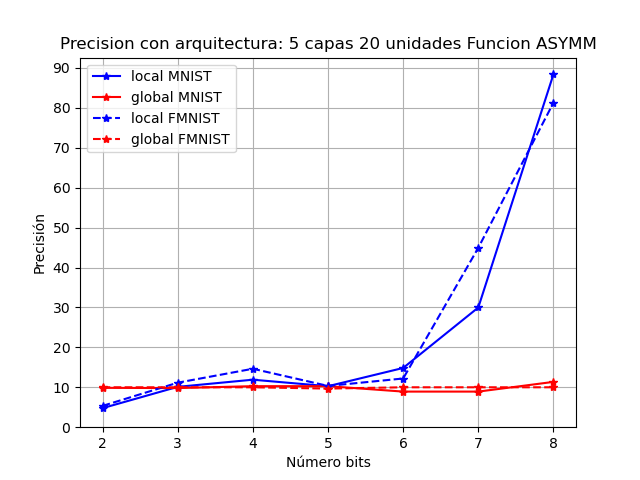
\includegraphics[width=\textwidth]{imagenes/HSIC/Precision con arquitectura: 5 capas 20 unidades Funcion ASYMM.png}
    \end{subfigure}
    \begin{subfigure}[H]{0.475\textwidth}
    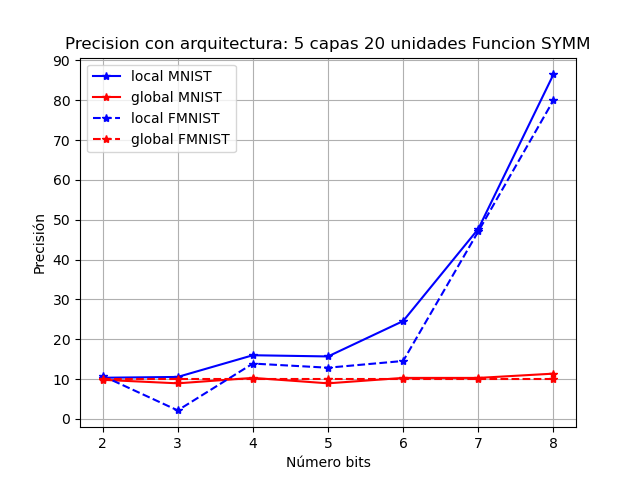
\includegraphics[width=\textwidth]{imagenes/HSIC/Precision con arquitectura: 5 capas 20 unidades Funcion SYMM.png}
    \end{subfigure}

    %\label{fig:my_label}
\end{figure}
Al igual que en el modelo base, no hay mucha diferencia entre ambas funciones de cuantificación. Y como ocurría con el Backpropagation, profundidades más elevadas hacen imposible la aplicación de la cuantificación a nivel global. Por su parte, los modelos con cuantificación local, haciendo uso de 8 bits, consiguen mejorar los resultados del modelo base. Por lo tanto, ese aumento de profundidad permite mejorar los resultados de la red a nivel local, mientras que el nivel global es inviable.

Ahora vamos a analizar como afecta al algoritmo un aumento considerable de la anchura del modelo, empezando por los modelos con 2 capas ocultas y 50 y 100 neuronas.

\begin{figure}[H]
    \centering
    \begin{subfigure}[H]{0.475\textwidth}
    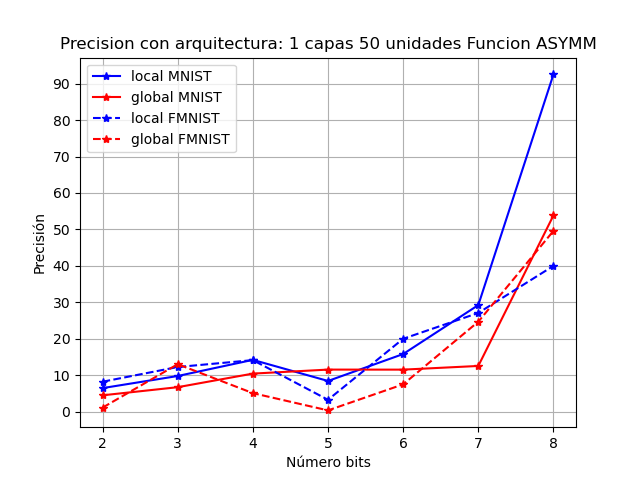
\includegraphics[width=\textwidth]{imagenes/HSIC/Precision con arquitectura: 1 capas 50 unidades Funcion ASYMM.png}
    \end{subfigure}
    \begin{subfigure}[H]{0.475\textwidth}
    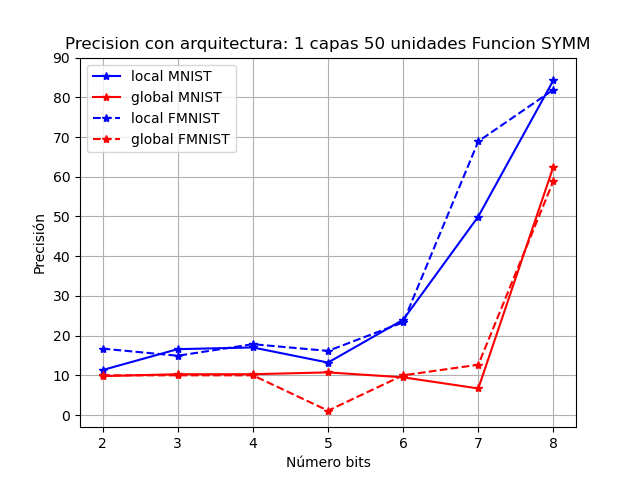
\includegraphics[width=\textwidth]{imagenes/HSIC/Precision con arquitectura: 1 capas 50 unidades Funcion SYMM.png}
    \end{subfigure}
    \begin{subfigure}[H]{0.475\textwidth}
    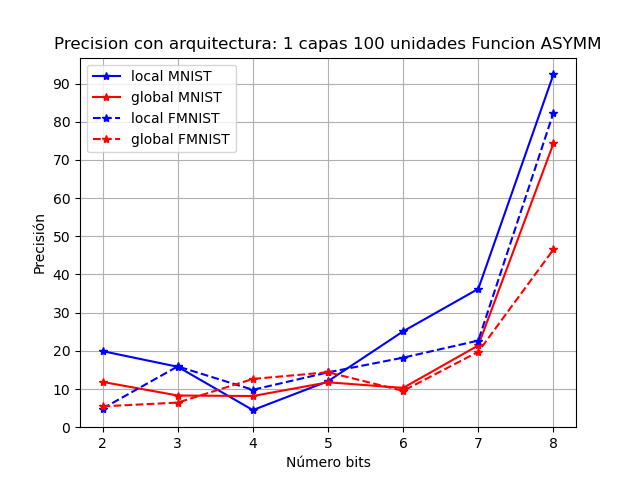
\includegraphics[width=\textwidth]{imagenes/HSIC/Precision con arquitectura: 1 capas 100 unidades Funcion ASYMM.png}
    \end{subfigure}
    \begin{subfigure}[H]{0.475\textwidth}
    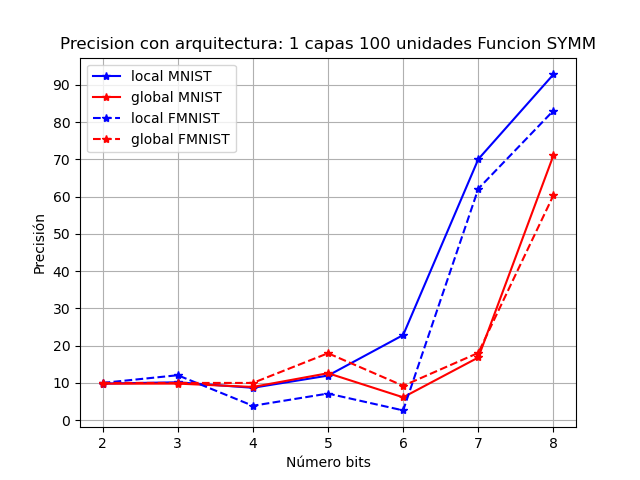
\includegraphics[width=\textwidth]{imagenes/HSIC/Precision con arquitectura: 1 capas 100 unidades Funcion SYMM.png}
    \end{subfigure}
    \caption{Arquitectura: 2 capas ocultas}
    %\label{fig:my_label}
\end{figure}

Con arquitectura más grandes, podemos observar que los modelos que usan la función de cuantificación SYMM consiguen mejores resultados. Esta diferencia se nota cuando se llega a los 8 bits, pues por debajo de este umbral, el algoritmo no es capaz de alcanzar buenos resultados. Además, con esta función, se consiguen prácticamente las mismas precisiones en ambos problemas. Con respecto al aumento de la anchura, vemos que la diferencia se nota en los 8 bits. En este caso, los resultados alcanzados por la cuantificación local superan en un 20\% a los alcanzados por la cuantificación global. Y por su parte, la cuantificación global, consigue mejores resultados con el aumento de la anchura.

\newpage
Ahora vamos a ver lo que ocurre cuando añadimos una capa extra.

\begin{figure}[H]
    \centering
    \begin{subfigure}[H]{0.475\textwidth}
    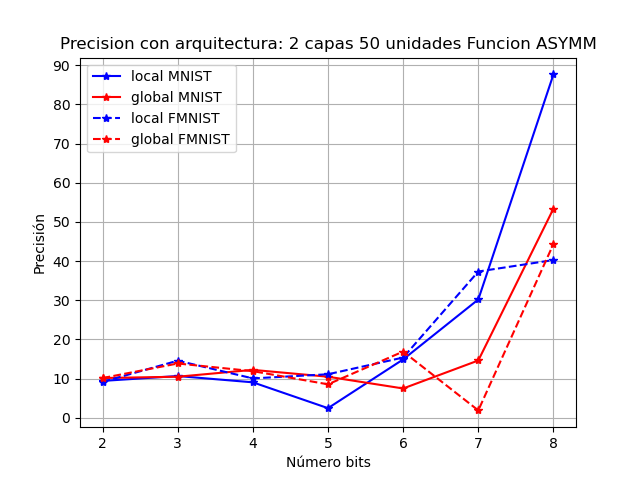
\includegraphics[width=\textwidth]{imagenes/HSIC/Precision con arquitectura: 2 capas 50 unidades Funcion ASYMM.png}
    \end{subfigure}
    \begin{subfigure}[H]{0.475\textwidth}
    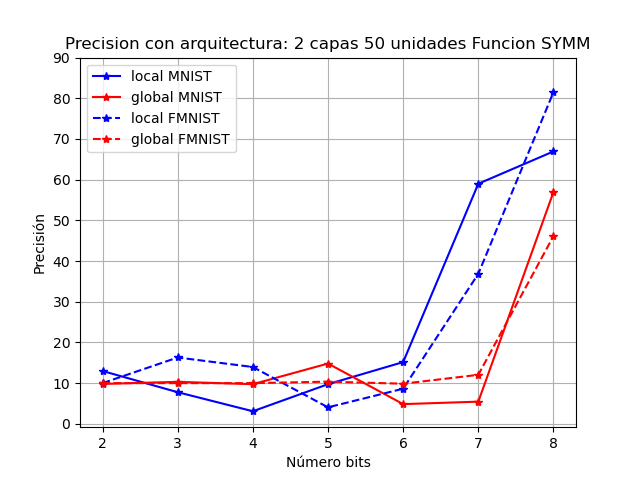
\includegraphics[width=\textwidth]{imagenes/HSIC/Precision con arquitectura: 2 capas 50 unidades Funcion SYMM.png}
    \end{subfigure}
    \begin{subfigure}[H]{0.475\textwidth}
    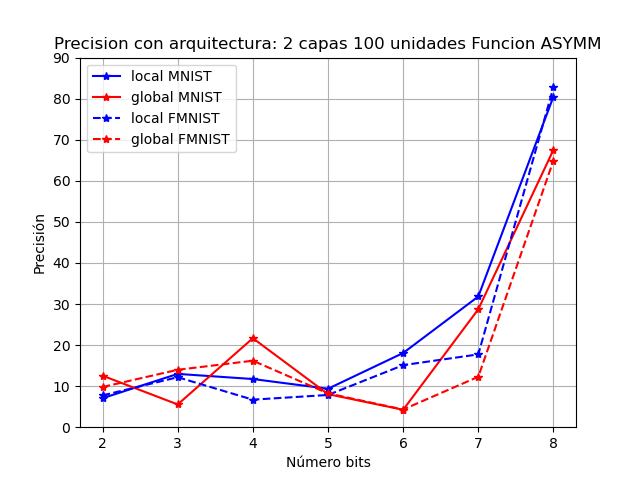
\includegraphics[width=\textwidth]{imagenes/HSIC/Precision con arquitectura: 2 capas 100 unidades Funcion ASYMM.png}
    \end{subfigure}
    \begin{subfigure}[H]{0.475\textwidth}
    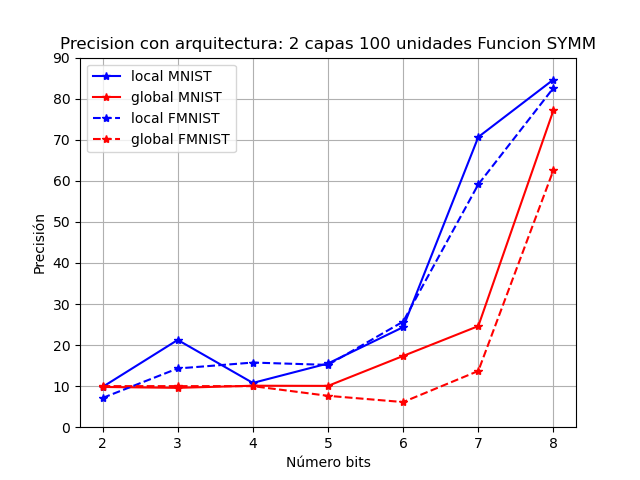
\includegraphics[width=\textwidth]{imagenes/HSIC/Precision con arquitectura: 2 capas 100 unidades Funcion SYMM.png}
    \end{subfigure}
    \caption{Arquitectura: 2 capas ocultas}
    %\label{fig:my_label}
\end{figure}

Estos modelos consiguen resultados muy parecidos a los alcanzados por los modelos de 2 capas. Para los modelos que usan la función ASYMM, los resultados son prácticamente idénticos, siendo la mayor diferencia: la mejora de precisión del modelo de 8 bits con cuantificación global sobre FMNIST, consiguiendo mejorar un 20\%. Es en los modelos que se han cuantificado con SYMM donde podemos encontrar más diferencias. En los modelos con anchura de 50 neuronas, los modelos con cuantificación global pierden precisión en comparación con los modelos de una capa oculta menos. Además, con cuantificación local, se ha conseguido mejores resultado sobre FMNIST que con MNIST, esto se ha podido dar por el sobreentrenamiento. Aumentar la complejidad de la red ha permitido mantener la precisión en el problema FMNIST, pero provoca un sobreajuste en el problema MNIST. Cuando se aumenta la anchura a 100 unidades por capa, se consigue mejorar la precisión de todos los modelos. En los modelos cuantificados con ASYMM: se consigue mejorar los resultados de los modelos cuantificados a nivel local, se aumenta la precisión en FMNIST y en MNIST decae ligeramente la precisión. Por su parte, los modelos cuantificados con SYMM consiguen mejores resultados cuando usan 7 bits. Con 8 bits los resultados son casi idénticos, consiguiendo una ligera mejora en los modelos cuantificados globalmente.

\newpage

\section{FeedbackAlignment}

A continuación, analizaremos el comportamiento del algoritmo de FeedbackAlignment.

\subsection{Arquitectura base}

\begin{figure}[H]
    \centering
    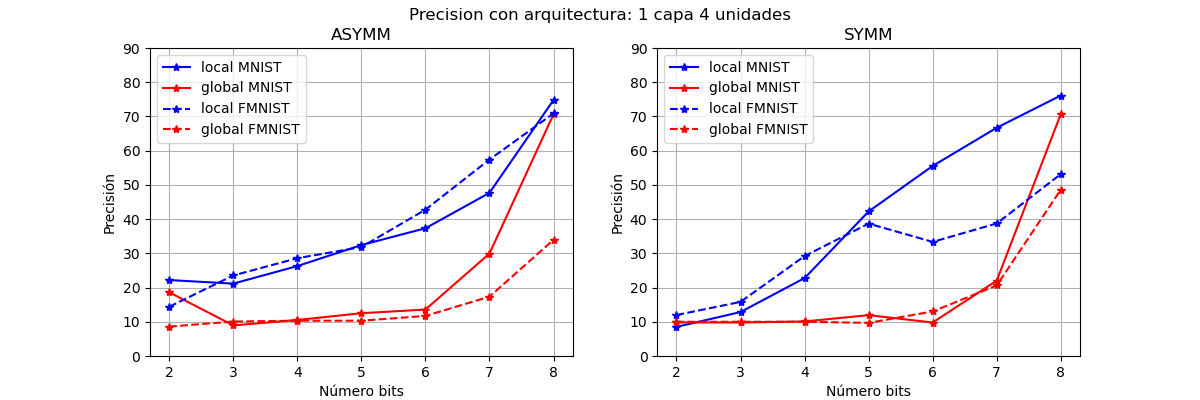
\includegraphics[width=\textwidth]{imagenes/fa/Precision con arquitectura: 1 capa 4 unidades.png}
    \caption{ASYMM vs SYMM}
    %\label{fig:asymmvssymmHSIC}
\end{figure}

Empecemos por analizar el comportamiento de los modelos cuantificados con ASYMM. Para los modelos locales, vemos que este algoritmo ofrece precisiones muy parecidas en ambos problemas. Conforme aumenta el número de bits aumenta la precisión obtenida, llegando al 70\% en ambos problemas con los 8 bits de precisión. Por su parte, en los modelos con cuantificación global,  la precisión obtenida con 8 bits en MNIST iguala prácticamente a la alcanzada por los modelos locales, mientras que en FMNIST, no se consigue superar el 40\% de precisión.  

Ahora pasamos a lo modelos cuantificados con la función SYMM. Los modelos cuantificados con esta función mejora los resultados obtenidos en MNIST, consiguiendo mejores resultados con menor cantidad de bits. Sin embargo, en FMNIST, los resultados de los modelos cuantificados localmente disminuyen, cayendo casi al 50\% con 8 bits, mientras que los cuantificados globalmente aumentan llegando prácticamente a esta precisión. Por lo tanto, con el modelo base, ASYMM funciona mejor para FMNIST, mientras que para MNIST es mejor usar SYMM.


\newpage

\subsection{Arquitecturas grandes}
Analizado el comportamiento del modelo base, toca analizar como afecta el aumento de la profundidad y anchura de las redes.

Como en los anteriores algoritmos, lo primero que vamos a analizar es como afecta aumentar la profundidad de la red.
\begin{figure}[H]
    \centering
    \begin{subfigure}[H]{0.475\textwidth}
    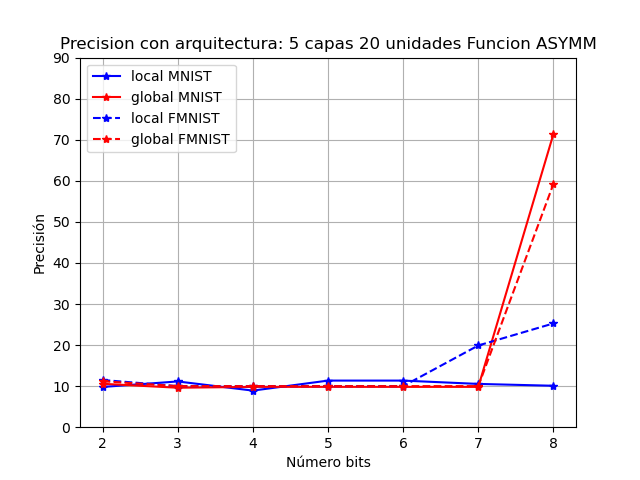
\includegraphics[width=\textwidth]{imagenes/fa/Precision con arquitectura: 5 capas 20 unidades Funcion ASYMM.png}
    \end{subfigure}
    \begin{subfigure}[H]{0.475\textwidth}
    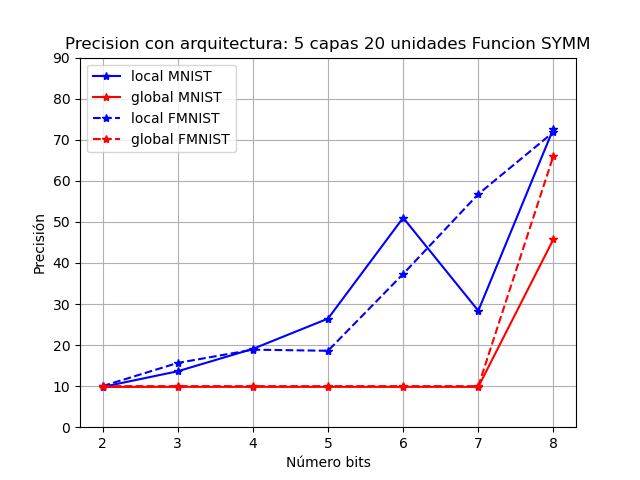
\includegraphics[width=\textwidth]{imagenes/fa/Precision con arquitectura: 5 capas 20 unidades Funcion SYMM.png}
    \end{subfigure}
    %\label{fig:my_label}
\end{figure}

Viendo las gráficas podemos apreciar que los resultados no son muy positivos. Empecemos por los modelos cuantificados por ASYMM. La cuantificación local es inviable, el ruido introducido por el algoritmo hace imposible superar el 30\% de precisión, lo que supone un resultado de un clasificador prácticamente aleatorio. La cuantificación local, en cambio, consigue con 8 bits precisiones del 70\% para MNIST y 60\% para FMNIST. No son resultados muy buenos pero superan considerablemente a los locales. Una posible razón de esta mejora, es que la restricción sobre los pesos haya actuado como regulador, permitiendo alcanzar mejores resultados sin divergir. Fijémonos ahora en los modelos cuantificados con la función SYMM. Ahora los modelos locales consiguen los mejores resultados. Llegado a los 8 bits se consigue un 70\% de precisión en ambos  problemas. Los modelos globales por su parte, no consiguen precisiones muy elevadas. Con 8 bits se consigue casi un 70\% de precisión en FMNIST. Este valor no hay que tenerlo muy en cuenta ya que con 1 bit menos no se ha conseguido pasar del 10\% de precisión. Por lo que posiblemente ese casi 70\% se haya podido alcanzar debido a factores aleatorios, como el ruido introducido por la cuantificación.

A continuación, vamos a ver como afecta el aumento de la profundidad a este algoritmo. Comenzaremos con las arquitecturas de 2 capas ocultas.


\begin{figure}[H]
    \centering
    \begin{subfigure}[H]{0.475\textwidth}
    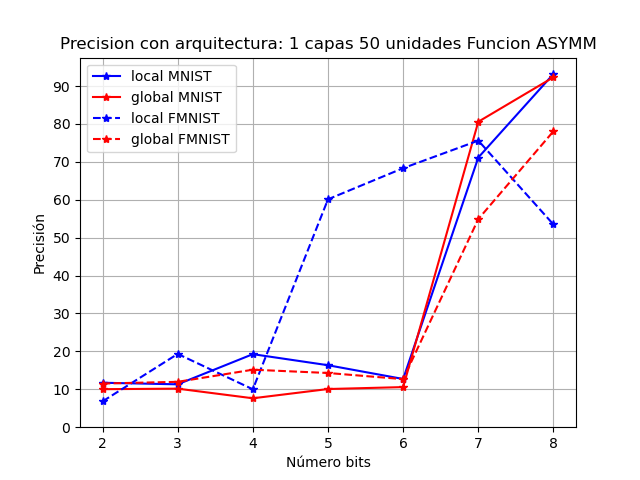
\includegraphics[width=\textwidth]{imagenes/fa/Precision con arquitectura: 1 capas 50 unidades Funcion ASYMM.png}
    \end{subfigure}
    \begin{subfigure}[H]{0.475\textwidth}
    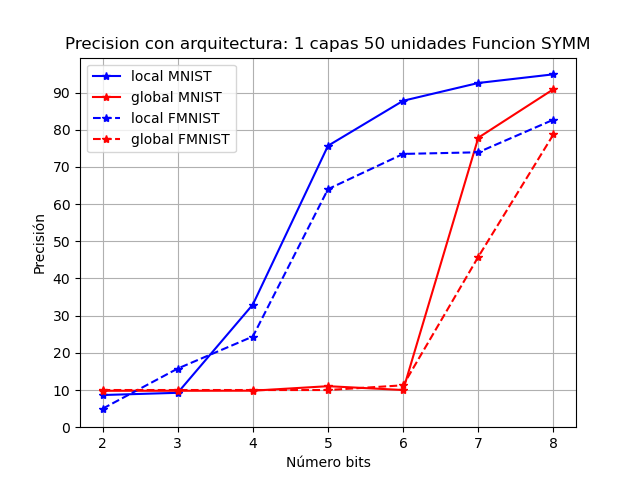
\includegraphics[width=\textwidth]{imagenes/fa/Precision con arquitectura: 1 capas 50 unidades Funcion SYMM.png}
    \end{subfigure}
    \begin{subfigure}[H]{0.475\textwidth}
    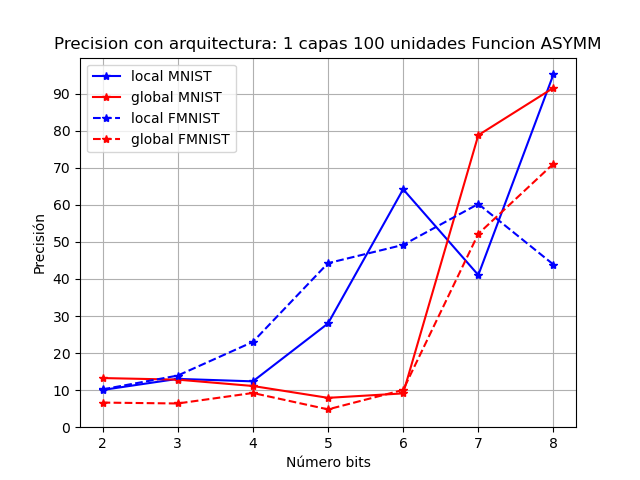
\includegraphics[width=\textwidth]{imagenes/fa/Precision con arquitectura: 1 capas 100 unidades Funcion ASYMM.png}
    \end{subfigure}
    \begin{subfigure}[H]{0.475\textwidth}
    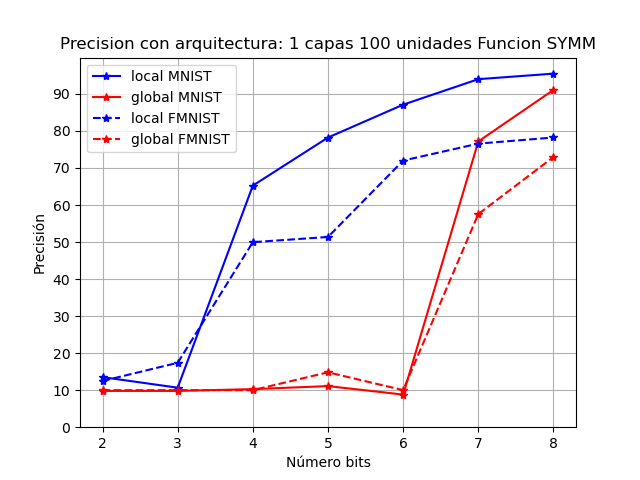
\includegraphics[width=\textwidth]{imagenes/fa/Precision con arquitectura: 1 capas 100 unidades Funcion SYMM.png}
    \end{subfigure}
    \caption{Arquitectura: 2 capas ocultas}
    %\label{fig:my_label}
\end{figure}

A primera vista, se puede apreciar que este algoritmo es mejor en redes más anchas que profundas. Vamos primero a analizar los modelos con anchura de 50 y después las de 100.

Viendo ambas gráficas, podemos ver que el aumento del número de bits supone una mejora en la precisión. A excepción del modelo local con 8 bits en el problema FMNIST. En este caso lo más seguro es que debido al aumento de precisión, el ruido introducido sea susceptible de alterar el comportamiento de la red, y por lo tanto, provocar que diverja y no alcance óptimos. El modelo global de 8 bits consigue mejores resultados en FMNIST, posiblemente debido a la restricción de pesos, que funciona como regulador. En MNIST, sin embargo, ambos niveles de cuantificación consiguen resultados en torno al 90\% con 8 bits de cuantificación. Si reducimos la precisión a 7 bits se consiguen resultados más o menos elevados, siendo el modelo cuantificado globalmente (80\% precisión) ligeramente superior al cuantificado localmente (70\% precisión).

Centrémonos ahora en los modelos cuantificados con SYMM. Todos los modelos mejoran al aumentar el número de bits, llegando a alcanzar el 90\% de precisión en MNIST y el 75-80\% en FMMIST. Con 8 bits se consiguen los mismos resultados que en los modelos cuantificados con ASYMM, con la diferencia de que: el modelo cuantificado localmente consigue mejorar hasta alcanzar el 75\% de precisión. Donde hay una clara mejora es en los modelos cuantificados localmente con 8 bits, superando el 70\% en ambos problemas a partir de los 6 bits. Por su parte, los modelos cuantificados localmente siguen necesitando mayor número de bits (7 bits en MNIST y 8 en FMNIST) para alcanzar valores buenos.

Aumentando la anchura a 100 bits podemos ver que las precisiones mejoran. Para los modelos cuantificados con ASYMM vemos como por debajo de los 8 bits los resultados mejoran, pero siguen siendo resultados bastante pésimos. Con 8 bits de precisión, los resultados se mantienen. Si pasamos a los modelos cuantificados con SYMM podemos apreciar una mejoría. Los modelos entre 5-8 bits mantienen las mismas precisiones, mejorando ligeramente. Es con 4 bits donde se nota una mayor mejoría, aunque siguen sin llegar a precisiones muy altas.


Ahora veamos que es lo que ocurre cuando aumentamos la profundidad de la red en 1 capa.

\begin{figure}[H]
    \centering
    \begin{subfigure}[H]{0.475\textwidth}
    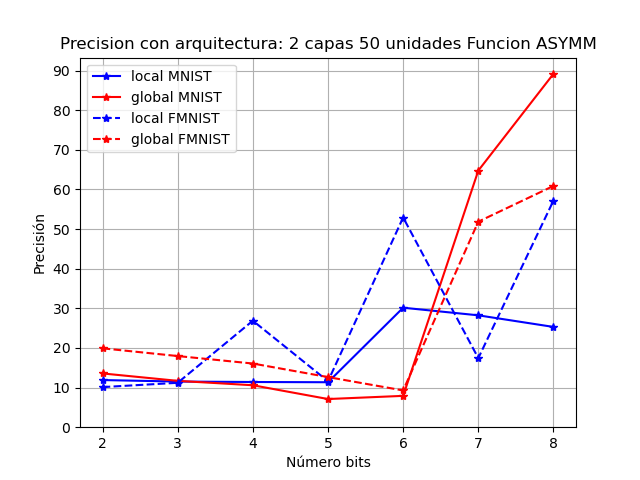
\includegraphics[width=\textwidth]{imagenes/fa/Precision con arquitectura: 2 capas 50 unidades Funcion ASYMM.png}
    \end{subfigure}
    \begin{subfigure}[H]{0.475\textwidth}
    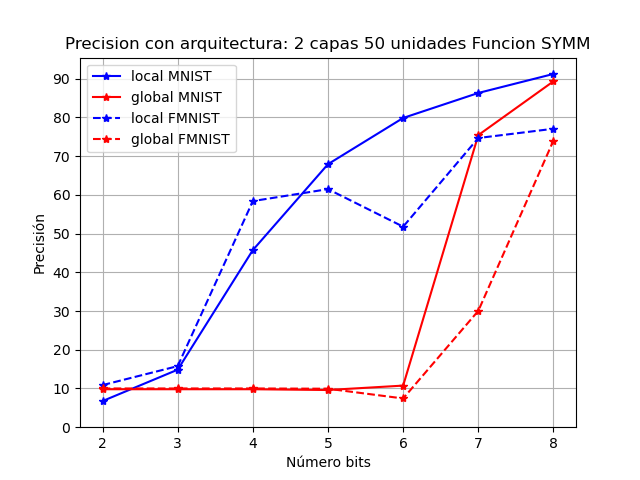
\includegraphics[width=\textwidth]{imagenes/fa/Precision con arquitectura: 2 capas 50 unidades Funcion SYMM.png}
    \end{subfigure}
    \begin{subfigure}[H]{0.475\textwidth}
    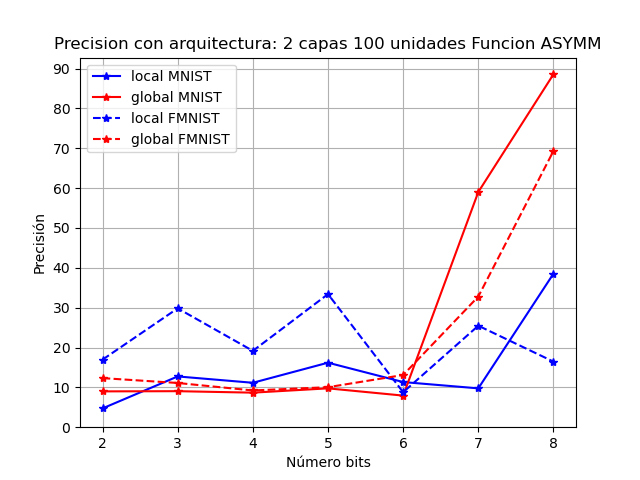
\includegraphics[width=\textwidth]{imagenes/fa/Precision con arquitectura: 2 capas 100 unidades Funcion ASYMM.png}
    \end{subfigure}
    \begin{subfigure}[H]{0.475\textwidth}
    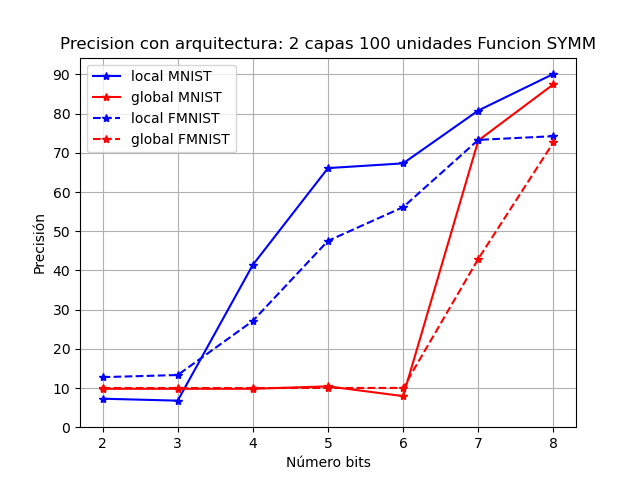
\includegraphics[width=\textwidth]{imagenes/fa/Precision con arquitectura: 2 capas 100 unidades Funcion SYMM.png}
    \end{subfigure}
    \caption{Arquitectura: 3 capas ocultas}
    %\label{fig:my_label}
\end{figure}

En los modelos que usan 50 unidades, más en específico los cuantificadas con ASYMM, podemos ver un empeoramiento de los resultados. Con los 8 bits se consiguen los mejores resultados, siendo los cuantificados globalmente los que mayor precisión alcanzan. En MNIST, se mantiene la precisión con el modelo cuantificado globalmente, pero el cuantificado localmente decae drásticamente a un 25\%. En FMNIST bajan los modelos cuantificados global y localmente. Pasando a los modelos cuantificados con la función SYMM, vemos que el comportamiento no varía mucho con respecto a los modelos con una capa menos. Cuando aumentamos la anchura a 100 unidades, podemos ver que los modelos cuantificados con ASYMM localmente empeoran su rendimiento, mientras que globalmente con 8 bits, mejoran ligeramente y con 7 bits empeoran. Por su parte, los cuantificados con SYMM no sufren gran cambio, consiguiendo precisiones muy parecidas.


\section{Synthetic gradients} \label{synthetic gradient}
Finalmente toca analizar el algoritmo de synthetic gradients.
\subsection{Modelo base}
\begin{figure}[H]
    \centering
    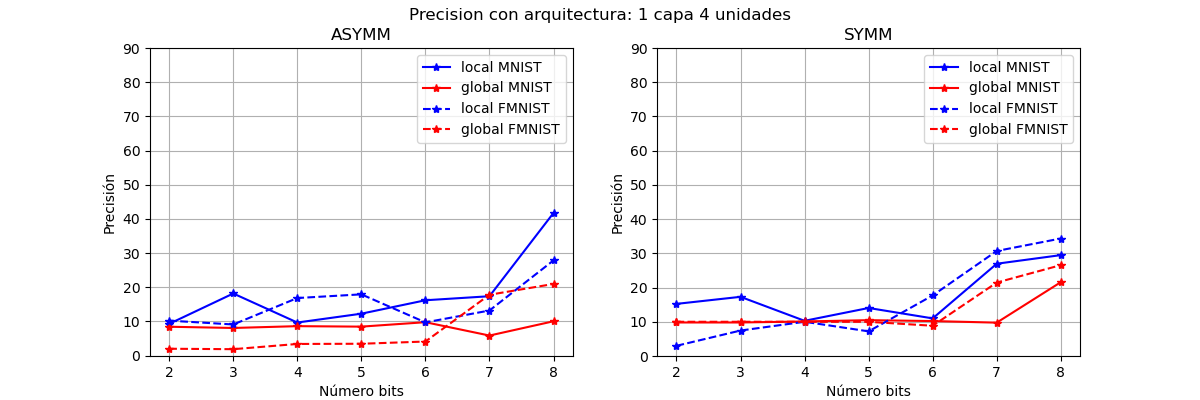
\includegraphics[width=\textwidth]{imagenes/dni/Precision con arquitectura: 1 capa 4 unidades.png}
    \caption{Arquitectura base}
    %\label{fig:asymmvssymmHSIC}
\end{figure}

Viendo ambas gráficas, podemos apreciar que este algoritmo es incapaz de resolver los problemas. Aún usando 8 bits, solo es capaz de llegar al 40\% de precisión en MNIST. Por lo tanto, con un modelo tan pequeño, aplicar synthetic gradient es inviable.


\subsection{Arquitecturas grandes}

Veamos ahora si aumentando el tamaño de la red se consiguen mejores resultados. Empecemos por aumentar la profundidad.

\begin{figure}[H]
    \centering
    \begin{subfigure}[H]{0.475\textwidth}
    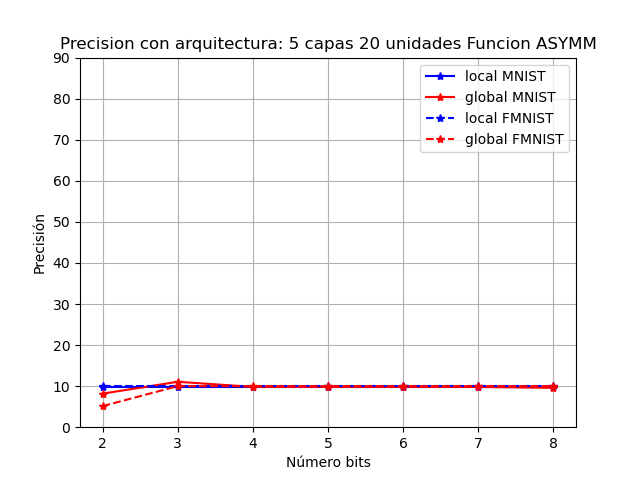
\includegraphics[width=\textwidth]{imagenes/dni/Precision con arquitectura: 5 capas 20 unidades Funcion ASYMM.png}
    \end{subfigure}
    \begin{subfigure}[H]{0.475\textwidth}
    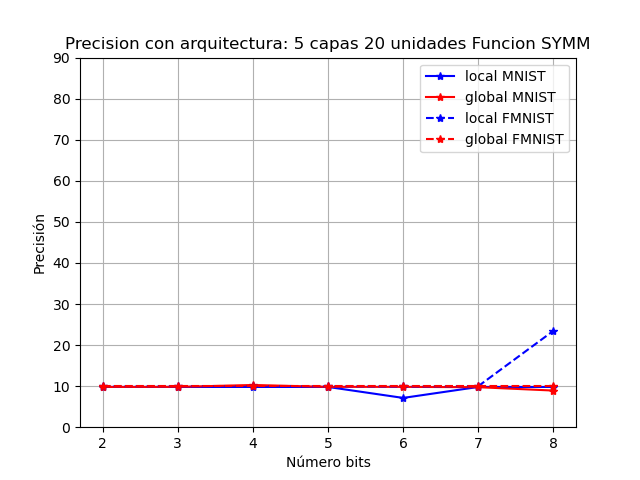
\includegraphics[width=\textwidth]{imagenes/dni/Precision con arquitectura: 5 capas 20 unidades Funcion SYMM.png}
    \end{subfigure}
    %\label{fig:my_label}
\end{figure}

Con este aumento de profundidad vemos que empeoran aun más los resultados. Todos los modelos obtienen un 10\% de precisión, lo que es equivalente a una clasificación aleatoria. El 20\% alcanzado en FMNIST no tiene mucho que destacar, ya que esta precisión también es propia de un clasificador aleatorio. Por lo tanto, con esta arquitectura también es imposible aplicar este algoritmo de entrenamiento. Veamos si con los modelos con más anchuras se consigue alguna mejora.

\begin{figure}[H]
    \centering
    \begin{subfigure}[H]{0.475\textwidth}
    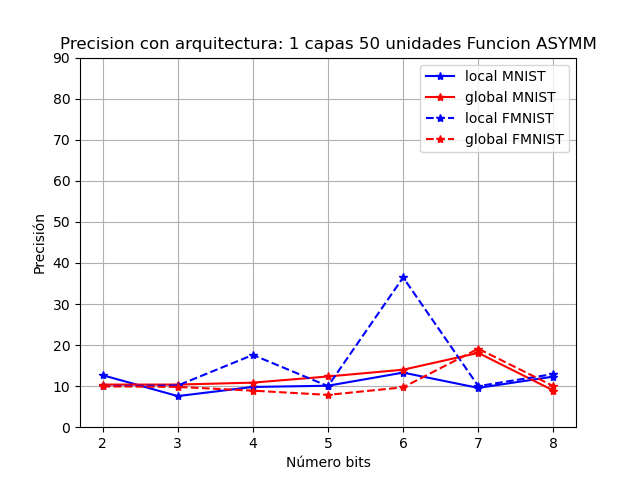
\includegraphics[width=\textwidth]{imagenes/dni/Precision con arquitectura: 1 capas 50 unidades Funcion ASYMM.png}
    \end{subfigure}
    \begin{subfigure}[H]{0.475\textwidth}
    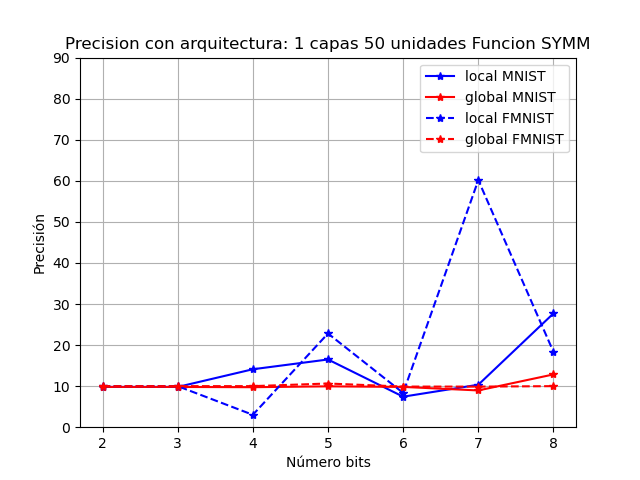
\includegraphics[width=\textwidth]{imagenes/dni/Precision con arquitectura: 1 capas 50 unidades Funcion SYMM.png}
    \end{subfigure}
    \begin{subfigure}[H]{0.475\textwidth}
    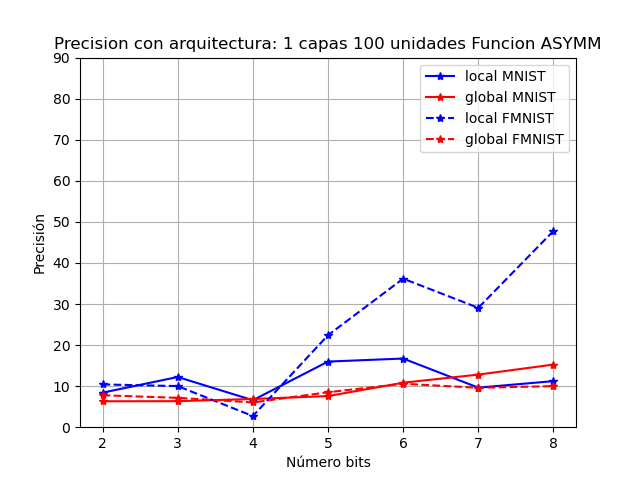
\includegraphics[width=\textwidth]{imagenes/dni/Precision con arquitectura: 1 capas 100 unidades Funcion ASYMM.png}
    \end{subfigure}
    \begin{subfigure}[H]{0.475\textwidth}
    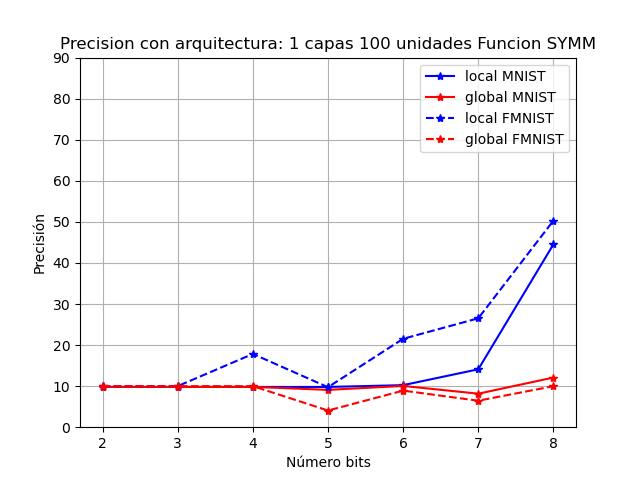
\includegraphics[width=\textwidth]{imagenes/dni/Precision con arquitectura: 1 capas 100 unidades Funcion SYMM.png}
    \end{subfigure}
    \caption{Arquitectura: 2 capas ocultas}
    %\label{fig:my_label}
\end{figure}

Con los modelos de 2 capas y 50 y 100 neuronas por capa oculta, podemos ver cierta mejora con respecto a la arquitectura anterior. Sin embargo, se siguen sin conseguir resultados decentes. Lo máximo que se alcanza es un 60\% en FMNIST con el modelo cuantificado con 7 bits localmente mediante SYMM. Se observa cierta mejora cuando se aumenta la anchura de la red, pero aun así, los resultados demuestran que en arquitecturas de este tamaño el algoritmo es inviable. Veamos por último, que ocurre si aumentamos en 1 capa la profundidad de la red. 

\begin{figure}[H]
    \centering
    \begin{subfigure}[H]{0.475\textwidth}
    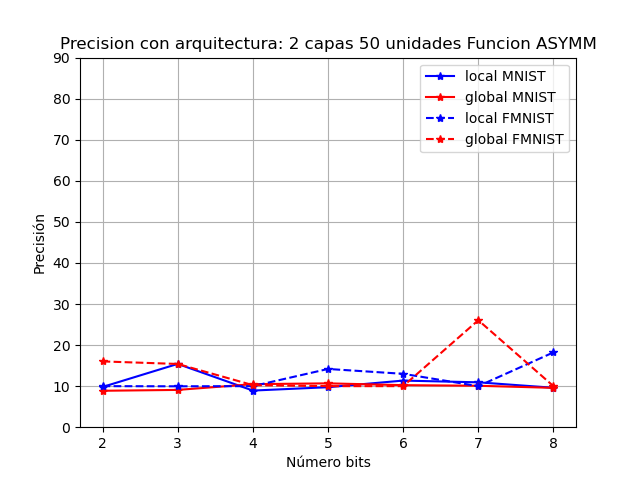
\includegraphics[width=\textwidth]{imagenes/dni/Precision con arquitectura: 2 capas 50 unidades Funcion ASYMM.png}
    \end{subfigure}
    \begin{subfigure}[H]{0.475\textwidth}
    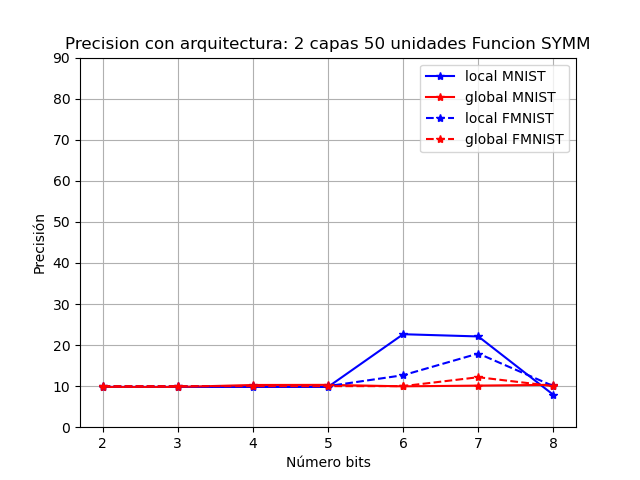
\includegraphics[width=\textwidth]{imagenes/dni/Precision con arquitectura: 2 capas 50 unidades Funcion SYMM.png}
    \end{subfigure}
    \begin{subfigure}[H]{0.475\textwidth}
    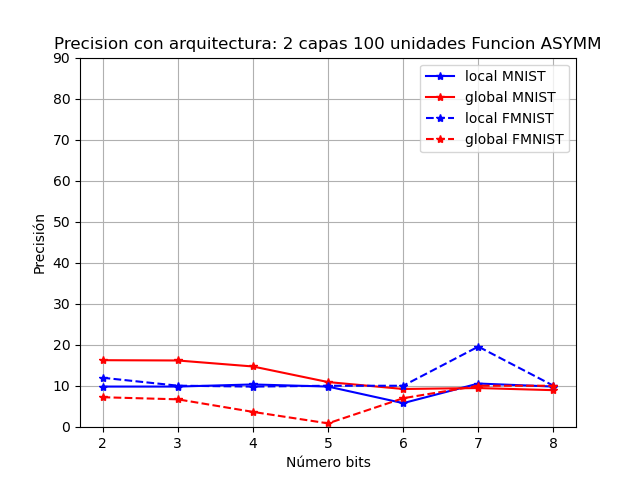
\includegraphics[width=\textwidth]{imagenes/dni/Precision con arquitectura: 2 capas 100 unidades Funcion ASYMM.png}
    \end{subfigure}
    \begin{subfigure}[H]{0.475\textwidth}
    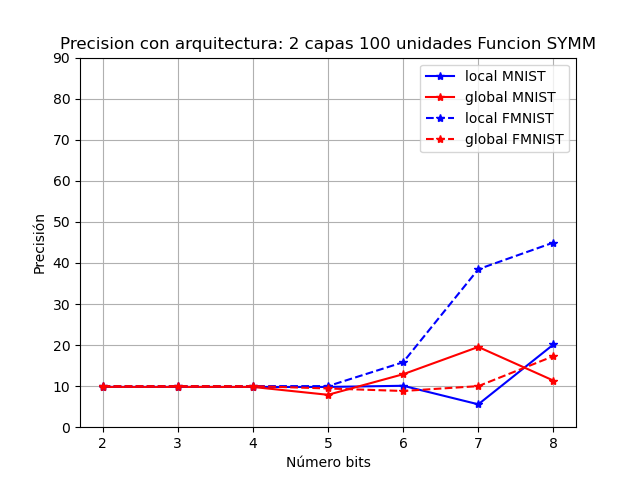
\includegraphics[width=\textwidth]{imagenes/dni/Precision con arquitectura: 2 capas 100 unidades Funcion SYMM.png}
    \end{subfigure}
    \caption{Arquitectura: 3 capas ocultas}
    %\label{fig:my_label}
\end{figure}

Una vez más, aumentada la profundidad, los resultados empeoran. El aumentar la anchura tampoco permite al algoritmo alcanzar mejores óptimos. Existe cierta mejoría, pero siguen siendo precisiones muy bajas. Por lo tanto, vemos que este algoritmo no es útil para redes en circuitos neuromórficos.